% --------------------------------------
% Document Class
% --------------------------------------
\documentclass[a4paper,11pt]{article}
% --------------------------------------



% --------------------------------------
% Use Package
% --------------------------------------


\usepackage[francais]{babel}
%\usepackage{ucs}
\usepackage[utf8]{inputenc}
\usepackage[T1]{fontenc}

\usepackage{makeidx}
\usepackage{color}
\usepackage{graphicx}
\usepackage{float}
\usepackage[hidelinks]{hyperref} 
\usepackage{geometry}
%\usepackage{lastpage}
%\usepackage{marginnote}
\usepackage{fancyhdr}
%\usepackage{titlesec}
%\usepackage{framed}
\usepackage{amsmath}
\usepackage{empheq}
\usepackage{array}
\usepackage{multicol}
\usepackage{csquotes}
%\usepackage{adjustbox}

% insert code
\usepackage{listings}

% define our color
\usepackage{xcolor}

% code color
\definecolor{ligthyellow}{RGB}{250,247,220}
\definecolor{darkblue}{RGB}{5,10,85}
\definecolor{ligthblue}{RGB}{1,147,128}
\definecolor{darkgreen}{RGB}{8,120,51}
\definecolor{darkred}{RGB}{160,0,0}

% other color
\definecolor{ivi}{RGB}{141,107,185}


\lstset{
    language=R,
    captionpos=b,
    extendedchars=true,
    frame=lines,
    numbers=left,
    numberstyle=\tiny,
    numbersep=5pt,
    keepspaces=true,
    breaklines=true,
    showspaces=false,
    showstringspaces=false,
    breakatwhitespace=false,
    stepnumber=1,
    showtabs=false,
    tabsize=3,
    basicstyle=\small\ttfamily,
    backgroundcolor=\color{ligthyellow},
    keywordstyle=\color{ligthblue},
    morekeywords={include, printf, uchar},
    identifierstyle=\color{darkblue},
    commentstyle=\color{darkgreen},
    stringstyle=\color{darkred},
}


% --------------------------------------



% --------------------------------------
% Page setting
% --------------------------------------
%\pagestyle{empty}
\setlength{\headheight}{15pt}

\setcounter{secnumdepth}{3}
\setcounter{tocdepth}{2}

\makeatletter
\@addtoreset{chapter}{part}
\makeatother 

\hypersetup{         % parametrage des hyperliens
  colorlinks=true,      % colorise les liens
  breaklinks=true,      % permet les retours à la ligne pour les liens trop longs
  urlcolor= blue,       % couleur des hyperliens
  linkcolor= black,     % couleur des liens internes aux documents (index, figures, tableaux, equations,...)
  citecolor= green      % couleur des liens vers les references bibliographiques
}

% --------------------------------------

% --------------------------------------
% Information
% --------------------------------------
\title{Compte-rendu TP5 RdF : Segmentation automatique par analyse d’histogramme}
\author{Elliot VANEGUE et Gaëtan DEFLANDRE}
% --------------------------------------

\definecolor{myColor}{rgb}{0.5, 0.1, 0.75}

% --------------------------------------
% Begin content
% --------------------------------------
\begin{document}

% Set language to english
  \selectlanguage{francais}

  % Start the page counting
  \pagenumbering{arabic}

  \maketitle
  
  \mbox{}
  \newpage
  \clearpage
  
  \section*{Introduction}
  Lors de ce TP, nous allons voir comment segmenter une image en niveau de gris en
  créant des macros avec le langage R. Nous utiliserons le seuillage automatique 
  de Bayes afin de voir les avantages et les inconvénients de cette méthode.
  
  % Lors de ce TP, nous allons voir comment automatiser la segmention d'une image en niveau de gris en 
  % utilisant le théorème de Bayes. Nous créerons des macros en language R 
  % afin de voir les avantages et les inconvénients de cette méthode.

  \section{Seuillage fixe}
  % nous avons testé plusieur seuils proches ..... , pour mettre en évidence l'importance de trouver un seuil précis. 
  Dans un premier temps, nous avons essayé trois seuils sur l'image \enquote{2classes\_100\_100\_8bits.png}.\\
  
  \begin{figure}[H]
    \center
    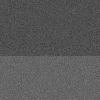
\includegraphics[width=5cm]{2classes_100_100_8bits.png}
    \caption{Image 2classes\_100\_100\_8bits.png}
  \end{figure}
  % Nous voyons que plus nous augmentons le seuil, plus le bruit est important dans la partie basse de l'image. 
  % Inversement, le bruit diminu dans la partie haute de l'image.
  Nous avons pu voir que plus nous augmentons le seuil et plus il y avait plus de bruit dans l'image
  binarisé sur la partie du bas de l'image. Et à l'inverse lorsque nous diminuons le seuil, le bruit 
  se ressens d'avantage sur la partie du haut de l'image.\\
  
  \begin{figure}[H]
    \center
    
\includegraphics[width=3cm]{resultat/bin35.png}
    
\includegraphics[width=3cm]{resultat/bin36.png}
    
\includegraphics[width=3cm]{resultat/bin37.png}
    \caption{Images binarisé avec un seuil de plus en plus grand}
  \end{figure}
  
  Dans nos résultats nous avons utilisé des seuils correspondant aux valeurs se trouvant dans le creux
  de l'histogramme de l'image que nous utilisons. Cela permet de séparer les deux pics lors de la 
  binarisation.\\
  
  \begin{figure}[H]
    \center
    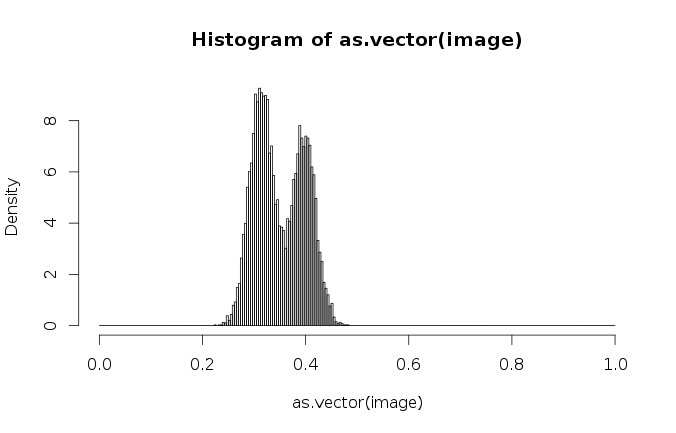
\includegraphics[width=10cm]{resultat/hist_image_principal.png}
    \caption{Histogramme de l'image 2classes\_100\_100\_8bits.png}
  \end{figure}
  
  
  % % Je sais pas, pour moi, on obtiendra le meilleur seuil avec Bayes, 
  % % et de manière automatique. Avec cette méthodes le seui est valide 
  % % que pour une image et c'est pas automatique. Mais je suis pas sur.
  % % Je pense pas que Bayes prend en compte la position et le voisinnage 
  % % des pixels, donc il ne corrigera pas les pixels de trop dans chaque classe.
  Donc le seuillage en utilisant l'histogramme de gris n'est pas la bonne solution pour 
  bien classer les pixels de l'image car les deux parties de celle-ci comporte des pixels
  dont le niveau de gris est similaire.
  
  \section{Seuillage automatique (Bayes) - Probabilité a priori des classes}
  Nous allons maintenant calculer la probabilité à priori des deux classes présentes dans l'image
  afin de pouvoir seuiller l'image grâce à la méthode de Bayes.\\
  
  Pour calculer cette probabilité, nous avons diviser le nombre de pixels d'une classe ($N_k$) par
  le nombre total de pixels ($N$). Ce qui nous donne les résultats suivants :
  $$\frac{N_{w_1}}{N} = 0.56$$
  $$\frac{N_{w_2}}{N} = 0.44$$\\
  
  Ce qui nous donne les macros suivante :\\
  
  \begin{lstlisting}[caption=Macros de calcule de probabilité à priori des classe $N_{w_1}$ et $N_{w_2}$]
  p_omega1= sum(h1$counts[0:255])/ sum(h$counts[0:255])
  p_omega2= sum(h2$counts[0:255])/ sum(h$counts[0:255])
  \end{lstlisting}
  
  \section{Seuillage automatique (Bayes) - Probabilité conditionnelle}
  Afin de calculer la probabilité d'erreur, nous avons besoin des probabilités conditionnelle des deux
  classes de l'image pour une valeur donnée. La valeur de X que nous avons utilisé durant nos calculs
  est 79. Nous devons diviser le nombre de pixels d'une classe d'un niveau de gris donné par le nombre total de
  pixels pour obtenir la probabilité conditionnelle. Ce qui nous donne les résulat suivant :
  
  $$P(79/I) = \frac{h(79)}{N} = 0.0362$$
  $$P(79/w_1) = \frac{h1(79)}{N} = 0.0362$$
  $$P(79/w_2) = \frac{h2(79)}{N} = 0$$\\
  
  Soit les macros suivante : \\
  
  \begin{lstlisting}[caption=Macros de calcule de probabilité à priori des classe $N_{w_1}$ et $N_{w_2}$]
  pI = h$counts[80] / sum(h$counts[0:255])
  pw1 = h1$counts[80] / sum(h$counts[0:255])
  pw2 = h2$counts[80] / sum(h$counts[0:255])
  \end{lstlisting}
  
  %TODO explication resultat 
  \section{Seuillage automatique (Bayes) - probabilité d’erreur}
  Nous allons maintenant calculer la probabilité d'erreur et effectuer une recherche de la 
  probabilité d'erreur minimum afin de trouver le seuil qui convient le mieu à l'image.
  Pour cela nous utilisons la macros suivante :
  
  \begin{lstlisting}[caption=Macros de calcule de probabilité à priori des classe $N_{w_1}$ et $N_{w_2}$]
  for (X in 1:255) 
  { 
    somme1[X+1] = sum( h1$density[(X+1):256]) / sum(h1$density[1:256] )
    somme1[X+1] = somme1[X+1] * p_omega1  
    somme2[X+1] = sum( h2$density[(X+1):256]) / sum(h2$density[1:256] )
    somme2[X+1] = somme2[X+1] * p_omega2

    erreur[X+1] = somme1[X+1] + somme2[X+1]
    
    # seuil corrrespondant à l'erreur minimale
    if (erreur[X+1] < minimum_erreur ) seuil_minimum_erreur = X
    if (erreur[X+1] < minimum_erreur ) minimum_erreur = erreur[X+1]
  }
  \end{lstlisting}
  
  
  \section{Extraction de la région représentant le 0 par seuillage automatique (Bayes)}
  
  \section{Seuillage automatique (Bayes) - Segmentation d’une image à 3 classes}
  
  \section{Taux d’erreur de classification}
  
  \section*{Conclusion}
  % Le problème avec Bayes c'est qu'on a besoin de connaitre l'histogramme de chacune des classes, donc pas très pratique
 
    
\end{document}  